\chapter{Referencial Teórico}
\section{Diabetes}
O diabetes mellitus é uma doença crônica caracterizada pela elevação persistente dos níveis de glicose no sangue, resultante de defeitos na produção e/ou ação da insulina. Os tipos mais comuns são o diabetes tipo 1, causado pela destruição autoimune das células beta pancreáticas; o tipo 2, associado à resistência à insulina e mais comum em adultos; e o diabetes gestacional, que ocorre durante a gravidez \cite{BRASIL2022}. Segundo a Organização Mundial da Saúde \cite{WHO2021}, o diabetes afeta centenas de milhões de pessoas em todo o mundo, sendo responsável por elevado ônus social e econômico devido às complicações crônicas, como doenças cardiovasculares, nefropatías, neuropatias e retinopatias. A detecção precoce é importante, já que intervenções no início do curso clínico da doença podem retardar ou prevenir complicações graves. Por isso, métodos preditivos ganham destaque como ferramentas de apoio à saúde pública.

\section{Machine Learning}
Segundo Andriy Burkov\cite{Burkov2020} em Machine Learning Engineering o aprendizado de Máquina (ML), é um subcampo dinâmico da inteligência artificial (IA), dedica-se ao desenvolvimento de sistemas que adquirem a capacidade de aprender com os dados. Em vez de depender de regras programadas explicitamente para cada cenário, esses sistemas são projetados para identificar padrões complexos, construir modelos preditivos e tomar decisões autônomas. Essa capacidade de "aprender" a partir da experiência, de forma semelhante ao processo cognitivo humano, é o que distingue o ML de abordagens computacionais mais tradicionais.

Tradicionalmente, as abordagens de ML são categorizadas em quatro paradigmas principais:

\subsection{Aprendizado Supervisionado}
Segundo Prado \cite{Prado2001}, no aprendizado supervisionado, os algoritmos são treinados com conjuntos de dados rotulados, ou seja, onde as entradas já possuem as saídas corretas associadas. O objetivo é que o algoritmo aprenda a mapear essas entradas para as saídas, generalizando esse conhecimento para novos dados não vistos. Exemplos incluem classificação, como podemos ver na figura \ref{fig:class_reg} temos o exemplo de predição de categorias discretas, como "doente" ou "saudável" e regressão predição de valores contínuos, como a pressão arterial. \cite{Feitosa2024}

\begin{figure}[H]
    \centering
    \caption{Diferença entre classificação e regressão}
    \label{fig:class_reg}
    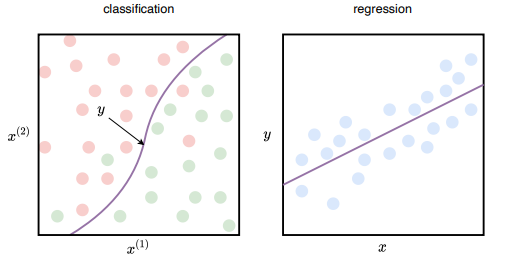
\includegraphics[width=0.8\textwidth]{../figuras/regression_classification.png} 
    \source{ (Burkov, 2020) }
\end{figure}

\subsection{Aprendizado Não Supervisionado}
Diferentemente do aprendizado supervisionado, no aprendizado não supervisionado, segundo Hastie e Friedman\cite{Hastie2009}, os dados utilizados nesta abordagem não possuem rótulos. O foco é descobrir estruturas ocultas, agrupamentos naturais ou padrões intrínsecos nos dados. Técnicas comuns incluem agrupamento, onde dados semelhantes são agrupados, e redução de dimensionalidade, que simplifica a representação dos dados mantendo suas características essenciais.

\subsection{Aprendizado Semi-Supervisionado}
Neste paradigma para Chapelle\cite{Chapelle2006} ele representa um meio-termo entre o aprendizado supervisionado e o não supervisionado. Ele se torna particularmente útil em cenários onde a rotulagem de dados é um processo caro e demorado. Utiliza uma pequena quantidade de dados rotulados em conjunto com uma grande quantidade de dados não rotulados para treinar o modelo. A ideia é que os dados não rotulados ajudem o algoritmo a aprender sobre a estrutura geral dos dados, enquanto os dados rotulados fornecem a âncora para a aprendizagem direcionada.

\subsection{Aprendizado por Reforço}
Inspirado na psicologia comportamental, o aprendizado por reforço envolve um agente que interage com um ambiente dinâmico para alcançar um objetivo específico. O agente aprende através de tentativas e erros, recebendo recompensas por ações desejáveis e penalidades por ações indesejáveis. O objetivo é que o agente aprenda uma política de ações que maximize a recompensa cumulativa ao longo do tempo. Esta abordagem é amplamente utilizada em robótica, jogos e sistemas de controle.

Conforme Mitchell \cite{Mitchell1997}, a premissa fundamental do ML é permitir que os sistemas aprendam sem serem explicitamente programados para cada tarefa específica. Esta capacidade de adaptação e inferência a partir de dados é o que torna o ML uma ferramenta tão poderosa e versátil em uma gama crescente de domínios.


\section{Machine Learning aplicado à Saúde}
No setor da saúde, o Machine Learning tem demonstrado um potencial transformador, revolucionando diversas áreas e prometendo melhorias significativas na eficiência e qualidade dos cuidados. De acordo com \cite{AlZubaidi2021}, algumas das aplicações mais proeminentes incluem:

\subsection{Classificação e Diagnóstico de Doenças}
Algoritmos de ML podem analisar grandes volumes de dados de pacientes como por exemplo sintomas, resultados de exames laboratoriais e histórico médico para poderem auxiliar no diagnóstico precoce e preciso de doenças, desde condições crônicas como diabetes e doenças cardíacas até tipos específicos de câncer isso pode auxiliar a intervenções mais rápidas e eficazes.

\subsection{Suporte à Decisão Clínica}
Sistemas baseados em ML podem fornecer aos médicos informações valiosas e insights acionáveis para auxiliar na tomada de decisões clínicas. Isso inclui a recomendação de tratamentos personalizados com base nas características individuais do paciente, a previsão de resultados de tratamentos e a identificação de pacientes em risco de complicações.

\subsection{Medicina Personalizada}
Ao analisar o perfil genético, o histórico de vida e os dados clínicos de um indivíduo, o ML pode possibilitar abordagens de tratamento personalizadas, otimizando a escolha de terapias e dosagens para maximizar a eficácia e minimizar os efeitos colaterais.

\subsection{Monitoramento de Pacientes e Saúde Preventiva}
Dispositivos vestíveis e sensores podem coletar dados contínuos sobre a saúde dos indivíduos. Algoritmos de ML podem analisar esses dados para monitorar o estado de saúde, prever a ocorrência de eventos adversos e fornecer alertas em tempo real, permitindo uma intervenção precoce e promovendo a saúde preventiva.

O Aprendizado de Máquina está se consolidando como uma ferramenta indispensável no avanço da saúde, prometendo um futuro onde o diagnóstico é mais rápido, o tratamento mais eficaz e a medicina mais personalizada e preventiva.


\section{Redes Neurais Artificiais}
Uma Rede Neural Artificial (RNA) é um sistema computacional concebido para emular o modo como o cérebro humano processa informações ao executar uma tarefa específica. A sua implementação pode ser física, com o uso de componentes eletrônicos, ou, mais frequentemente, realizada através de simulação em computadores digitais. Para atingir um desempenho robusto, esses sistemas dependem de uma vasta rede interconectada de unidades computacionais elementares, conhecidas como "neurônios" ou unidades de processamento \cite{Haykin2009}.

Através de um processamento distribuído entre seus neurônios, as RNAs conseguem solucionar problemas de alta complexidade, mesmo em cenários onde o comportamento das variáveis subjacentes não é totalmente conhecido \cite{Busnardo2024}. Uma das suas características centrais é a habilidade de aprendizado por meio de exemplos, seguida da capacidade de generalizar o conhecimento adquirido para novos dados. Isso resulta na criação de um modelo não-linear, o que torna sua aplicação em domínios como a análise espacial altamente eficiente \cite{Sporl2011}.

No que tange à topologia, a implementação de uma RNA requer a definição de múltiplos parâmetros estruturais, entre os quais para santos\cite{Santos2005} se destacam: 
\begin{itemize}
	\item O número de nós na camada de entrada, que corresponde à dimensionalidade dos dados que alimentam a rede, geralmente selecionadas pela sua importância para o problema
	\item A quantidade de camadas ocultas e o número de neurônios em cada uma delas. 
	\item O número de neurônios na camada de saída, que é ditado pelo formato esperado da resposta do modelo.
\end{itemize}
As RNAs são, essencialmente, algoritmos computacionais que utilizam um modelo matemático inspirado na estrutura de organismos inteligentes, permitindo uma representação simplificada do funcionamento cerebral em um computador. Similarmente ao cérebro, a RNA é capaz de aprender e de tomar decisões fundamentadas nesse aprendizado. Trata-se, portanto, de um esquema de processamento que armazena conhecimento adquirido por treinamento e o disponibiliza para a aplicação a que se destina \cite{Sporl2011}.

Conforme \cite{Haykin2009}, a analogia entre a rede neural e o cérebro humano se manifesta em dois aspectos fundamentais: 
\begin{itemize}
	\item o conhecimento é assimilado pela rede a partir de seu ambiente através de um processo de aprendizagem.
	\item As forças de conexão entre os neurônios, denominadas pesos sinápticos, são usadas para armazenar o conhecimento adquirido.
\end{itemize}
As redes neurais artificiais emergiram da generalização de modelos matemáticos de sistemas nervosos biológicos. Nessa abstração, os nós são chamados de neurônios, e as sinapses são modeladas como pesos nas conexões, que modulam o sinal de entrada de cada neurônio. A característica não-linear, inspirada nos neurônios biológicos, é introduzida por uma função de ativação, permitindo à rede modelar relações complexas \cite{Abraham2005}.

Na arquitetura básica de um neurônio artificial demonstrada na figura \ref{fig:rede_neural}, podemos observar que ele opera sobre sinais de entrada, os quais são valores numéricos ponderados pelos pesos sinápticos, podendo ser oriundos de outros neurônios ou de uma fonte inicial de dados \cite{Busnardo2024}.

\begin{figure}[H]
    \centering
    \caption{Ilustração de uma rede neural}
    \label{fig:rede_neural}
    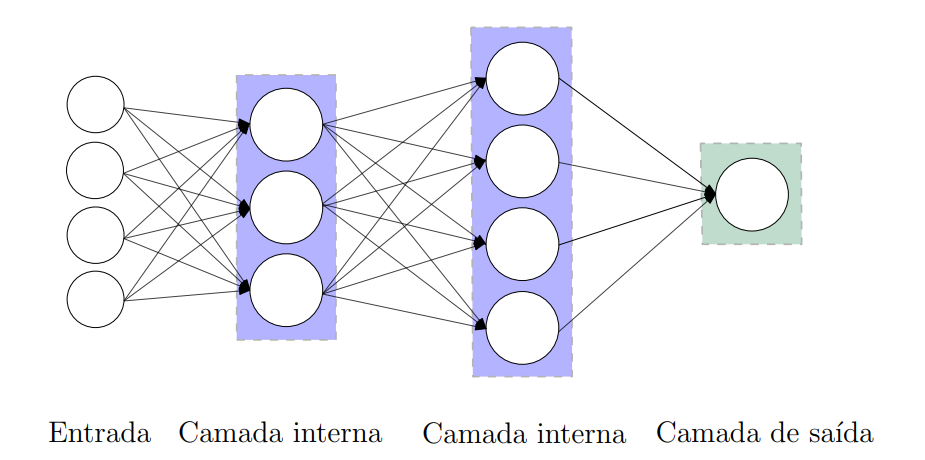
\includegraphics[width=0.8\textwidth]{figuras/a rede neural composta por três camadas.png} 
    \par 
    \small Fonte: (Kovaleski, 2018)
\end{figure}

O funcionamento de um neurônio artificial, conforme ilustrado na figura \ref{fig:rede_neural}, pode ser representado pela seguinte equação matemática:
$$ y = \phi\left(\sum_{i=1}^{n}\omega_i x_i + b\right) $$
Nesta expressão, $x_i$ representa os sinais de entrada, $\omega_i$ são os respectivos pesos sinápticos, $b$ é um valor de polarização, $\phi$ é a função de ativação aplicada à soma ponderada, e $y$ é o sinal de saída do neurônio \cite{Kovaleski2018}.

Segundo Busnardo \cite{Busnardo2024},os modelos que estruturam esses neurônios em camadas sequenciais são conhecidos como Multilayer Perceptron (MLP). Um MLP típico é composto por três tipos de camadas: a camada de entrada onde os sinais codificados são inseridos, as camadas ocultas onde os dados são processados e transformados e a camada de saída que gera o resultado final, como uma classificação.

Individualmente, um neurônio só é capaz de resolver problemas linearmente separáveis. A solução para problemas complexos exige a associação de múltiplos neurônios em várias camadas interconectadas. Essa abordagem de empilhamento de camadas é a base de arquiteturas mais sofisticadas, como as Redes Neurais Convolucionais \cite{Abraham2005}, que são pilares no campo do deep learning \cite{LeCun2015}.

\subsection{Z-Score}
O Z-Score segundo \cite{doi:10.1177/02537176211046525}, ou escore padrão, é uma técnica estatística essencial para a normalização de dados, utilizada para transformar variáveis de diferentes grandezas para uma mesma escala comparável, sem distorcer a distribuição original ou perder informações relativas aos intervalos. Matematicamente, o escore $z$ quantifica o número de desvios padrão que um ponto de dados específico se distancia da média, sendo calculado pela equação $z = \frac{x - \mu}{\sigma}$, onde $x$ representa o valor observado, $\mu$ a média da população e $\sigma$ o desvio padrão. A aplicação desse método resulta em uma distribuição com média zero e desvio padrão unitário, o que é particularmente crítico para o desempenho de algoritmos de aprendizado de máquina baseados em distância, além de constituir uma ferramenta robusta para a detecção de outliers, permitindo a identificação de observações anômalas que divergem estatisticamente do comportamento central dos dados.

\subsection{Smote}
O SMOTE (Synthetic Minority Over-sampling Technique) segundo \cite{rs11243040} destaca-se na literatura como uma das abordagens mais eficazes para mitigar o problema de desbalanceamento de classes em conjuntos de dados, uma condição que tende a enviesar modelos preditivos em favor da classe majoritária, prejudicando a sensibilidade em relação à classe de interesse. Diferentemente da sobreamostragem aleatória simples, que apenas replica registros existentes e pode levar ao overfitting, o SMOTE opera gerando dados sintéticos inéditos através de interpolação linear. O algoritmo seleciona exemplos da classe minoritária e identifica seus vizinhos mais próximos ($k$-nearest neighbors) no espaço de características; em seguida, cria novas instâncias sintéticas ao longo dos segmentos de reta que unem o exemplo atual aos seus vizinhos. Esse processo expande as regiões de decisão da classe minoritária de forma mais generalista, enriquecendo o conjunto de treinamento sem introduzir redundância exata.

\subsection{Funções De Ativação}
Diversas funções de ativação são empregadas, cada uma com suas características e adequações para diferentes cenários:

\subsubsection{Função Sigmóide}
Segundo \cite{Trask2019} a função sigmóide mapeia a entrada para um valor entre 0 e 1, sendo tradicionalmente usada em camadas de saída para problemas de classificação binária, onde a saída pode ser interpretada como uma probabilidade. No entanto, sofre do problema de "gradiente vanishing" para valores muito grandes ou muito pequenos, o que pode dificultar o treinamento de redes profundas. 
Podemos ver sua função na equação \ref{eq:Sigmóide}.
\begin{equation}
 \phi(x)= \frac{1}{1 +e^{-x}}
  \label{eq:Sigmóide}
 \end{equation}
Na figura \ref{fig:sig} podemos observar o gráfico da função sigmoid.

% Figura 3
\begin{figure}[H]
    \centering
    \caption{Gráfico da Função de Ativação Sigmóide.}
    \label{fig:sig}
    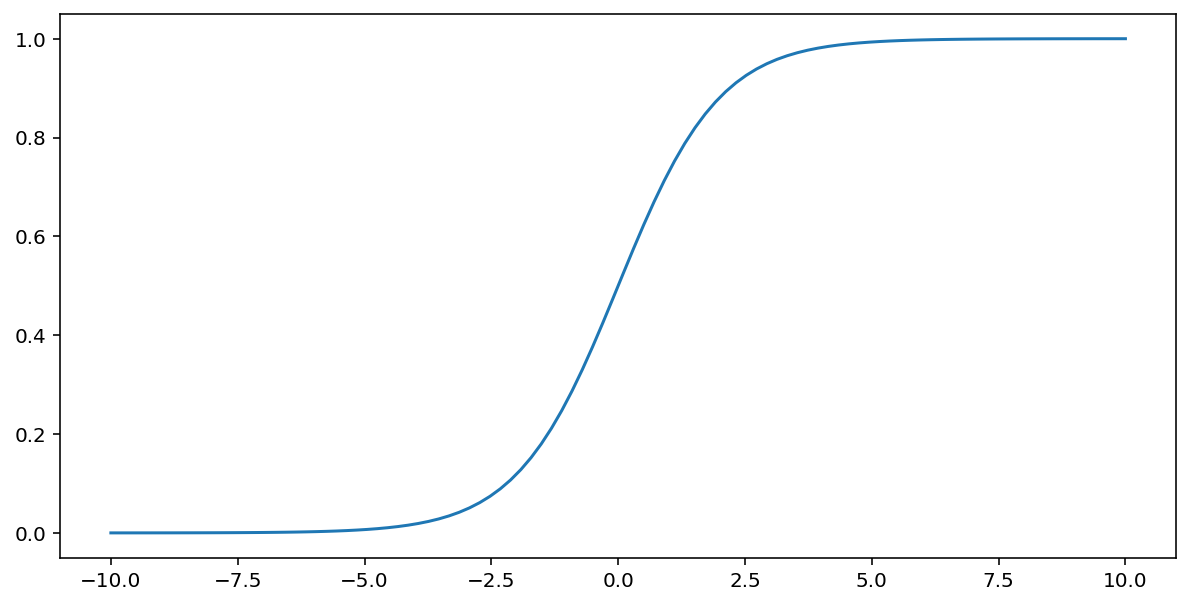
\includegraphics[width=0.8\textwidth]{figuras/graf_sigmoid.png} 
    \par 
    \small Fonte: (GOOGLE, 2025))
\end{figure}



\subsubsection{Função Tangente Hiperbólica (Tanh)}
Tanh é uma função de ativação frequentemente utilizada em redes neurais, notadamente por sua capacidade de escalar as saídas para o intervalo $[-1,1]$, o que contribui para a padronização dos valores de entrada. Sua característica de não-linearidade é fundamental, pois permite que a rede neural aborda problemas de classificação mais complexos, que não podem ser resolvidos por fronteiras lineares \cite{Goodfellow2016}. De acordo com \cite{Goodfellow2016}, a simetria do intervalo de saída em torno do zero é um fator que pode otimizar a velocidade de convergência do algoritmo de treinamento. Além disso, a derivabilidade da Tanh em todo o seu domínio simplifica significativamente o cálculo dos gradientes, um passo essencial no algoritmo de retropropagação. Por essas razões, a função de ativação Tanh é consistentemente uma escolha relevante em diversas aplicações de aprendizado de máquina com redes neurais.
Sua função é definida da seguinte forma:
\begin{equation}
 f(x) = \frac{e^x - e^{-x}}{e^x + e^{-x}}
  \label{eq:Tanh}
 \end{equation}
Abaixo na figura \ref{fig:tanh} podemos observar o gráfico da função Tanh.

\begin{figure}[H]
    \centering
    \caption{Gráfico da Função de Ativação Tangente Hiperbólica (Tanh).}
    \label{fig:tanh}
    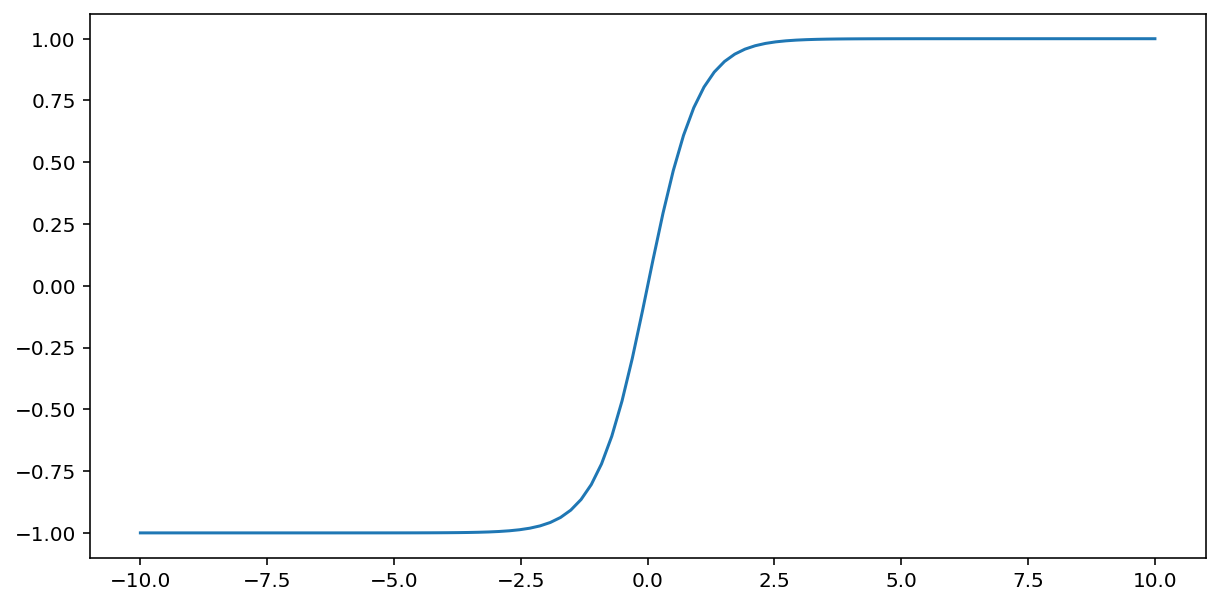
\includegraphics[width=0.8\textwidth]{figuras/tanh.png} 
    \par 
    \small Fonte: (GOOGLE, 2025))
\end{figure}

\subsubsection{Função ReLU (Rectified Linear Unit)}
Define a saída como o próprio valor de entrada se for positivo, e zero caso contrário. Essa função se tornou extremamente popular devido à sua simplicidade computacional e por mitigar o problema do gradiente vanishing para entradas positivas, acelerando o treinamento de redes profundas. No entanto, pode sofrer do problema "dying ReLU", onde neurônios podem se tornar inativos se suas entradas forem sempre negativas.
A função ReLU é definida pela seguinte função:
\begin{equation}
 f(x)=\max(0,x)
  \label{eq:ReLU}
 \end{equation}
Abaixo na figura \ref{fig:relu} podemos observar o gráfico da função ReLU.

\begin{figure}[H]
    \centering
    \caption{Gráfico da Função de Ativação ReLU.}
    \label{fig:relu}
    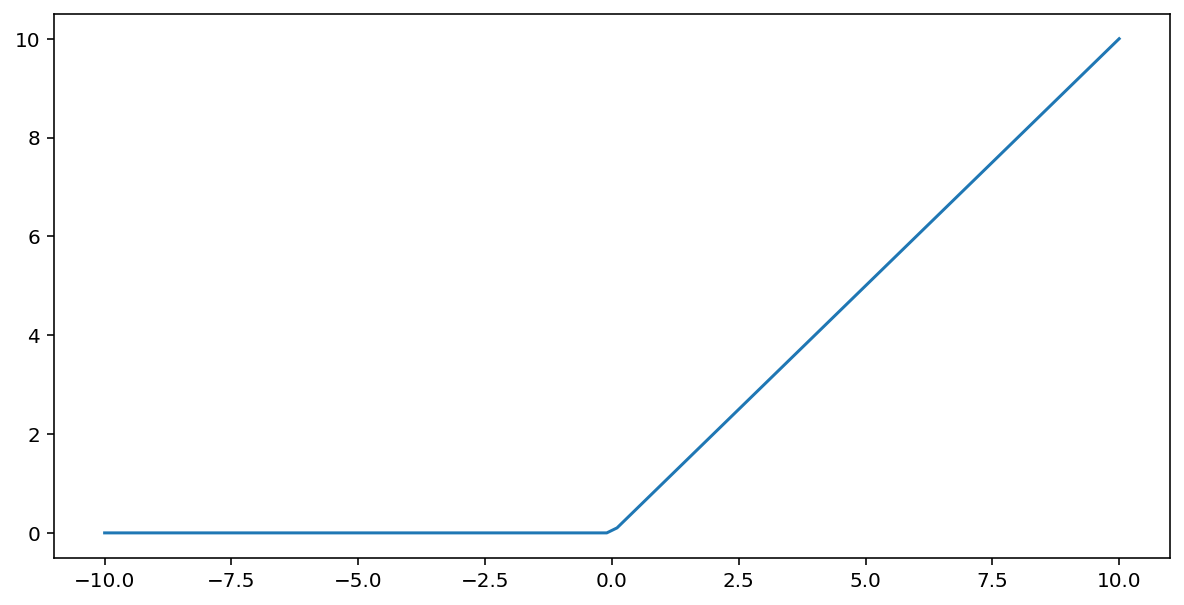
\includegraphics[width=0.8\textwidth]{figuras/relu.png} 
    \par 
    \small Fonte: (GOOGLE, 2025))
\end{figure}

\subsubsection{Qual Função De Ativação Utilizar}
A escolha da função de ativação impacta diretamente a capacidade de aprendizado e o desempenho da rede neural. As funções sigmóide e tanh foram dominantes no passado, mas a ReLU e suas variantes como Leaky ReLU, ELU, PReLU são atualmente as mais utilizadas em camadas ocultas de redes profundas, devido à sua eficiência no treinamento.

A versatilidade das RNAs é evidenciada pela diversidade de modelos e arquiteturas que se desenvolveram a partir desse conceito fundamental. O Perceptron de Múltiplas Camadas (MLP), por exemplo, é uma das formas mais básicas e amplamente utilizadas, consistindo em camadas totalmente conectadas capazes de aprender mapeamentos complexos. Com o avanço da capacidade computacional e a disponibilidade de grandes volumes de dados, surgiram as redes neurais profundas (Deep Neural Networks), que se caracterizam por possuírem múltiplas camadas ocultas, permitindo a extração de representações de dados em diferentes níveis de abstração. As Redes Neurais Convolucionais (CNNs), por sua vez, destacam-se em problemas que envolvem dados com estrutura de grade, como imagens e sinais, utilizando filtros convolucionais para detectar padrões locais. Outros modelos especializados, como as Redes Neurais Recorrentes (RNNs) e suas variações LSTM, GRU, são particularmente eficazes no processamento de sequências temporais, como texto e áudio. Esses modelos vêm sendo amplamente utilizados em problemas que envolvem grandes volumes de dados e alta dimensionalidade, onde métodos tradicionais poderiam falhar em identificar padrões sutis.

\section{IDE: PyCharm}
O PyCharm é uma das IDEs (Integrated Development Environment) mais renomadas para a programação em Python, desenvolvida pela JetBrains. Ela se destaca pela combinação de uma interface intuitiva que observamos na figura \ref{fig:pycharm} e uma ampla gama de recursos avançados, tornando-se uma ferramenta essencial para desenvolvedores de todos os níveis\cite{Jetbrains2025, Rocha2021, Pylinton2021}.

\begin{figure}[H]
    \centering
    \caption{Interface principal do PyCharm}
    \label{fig:pycharm}
    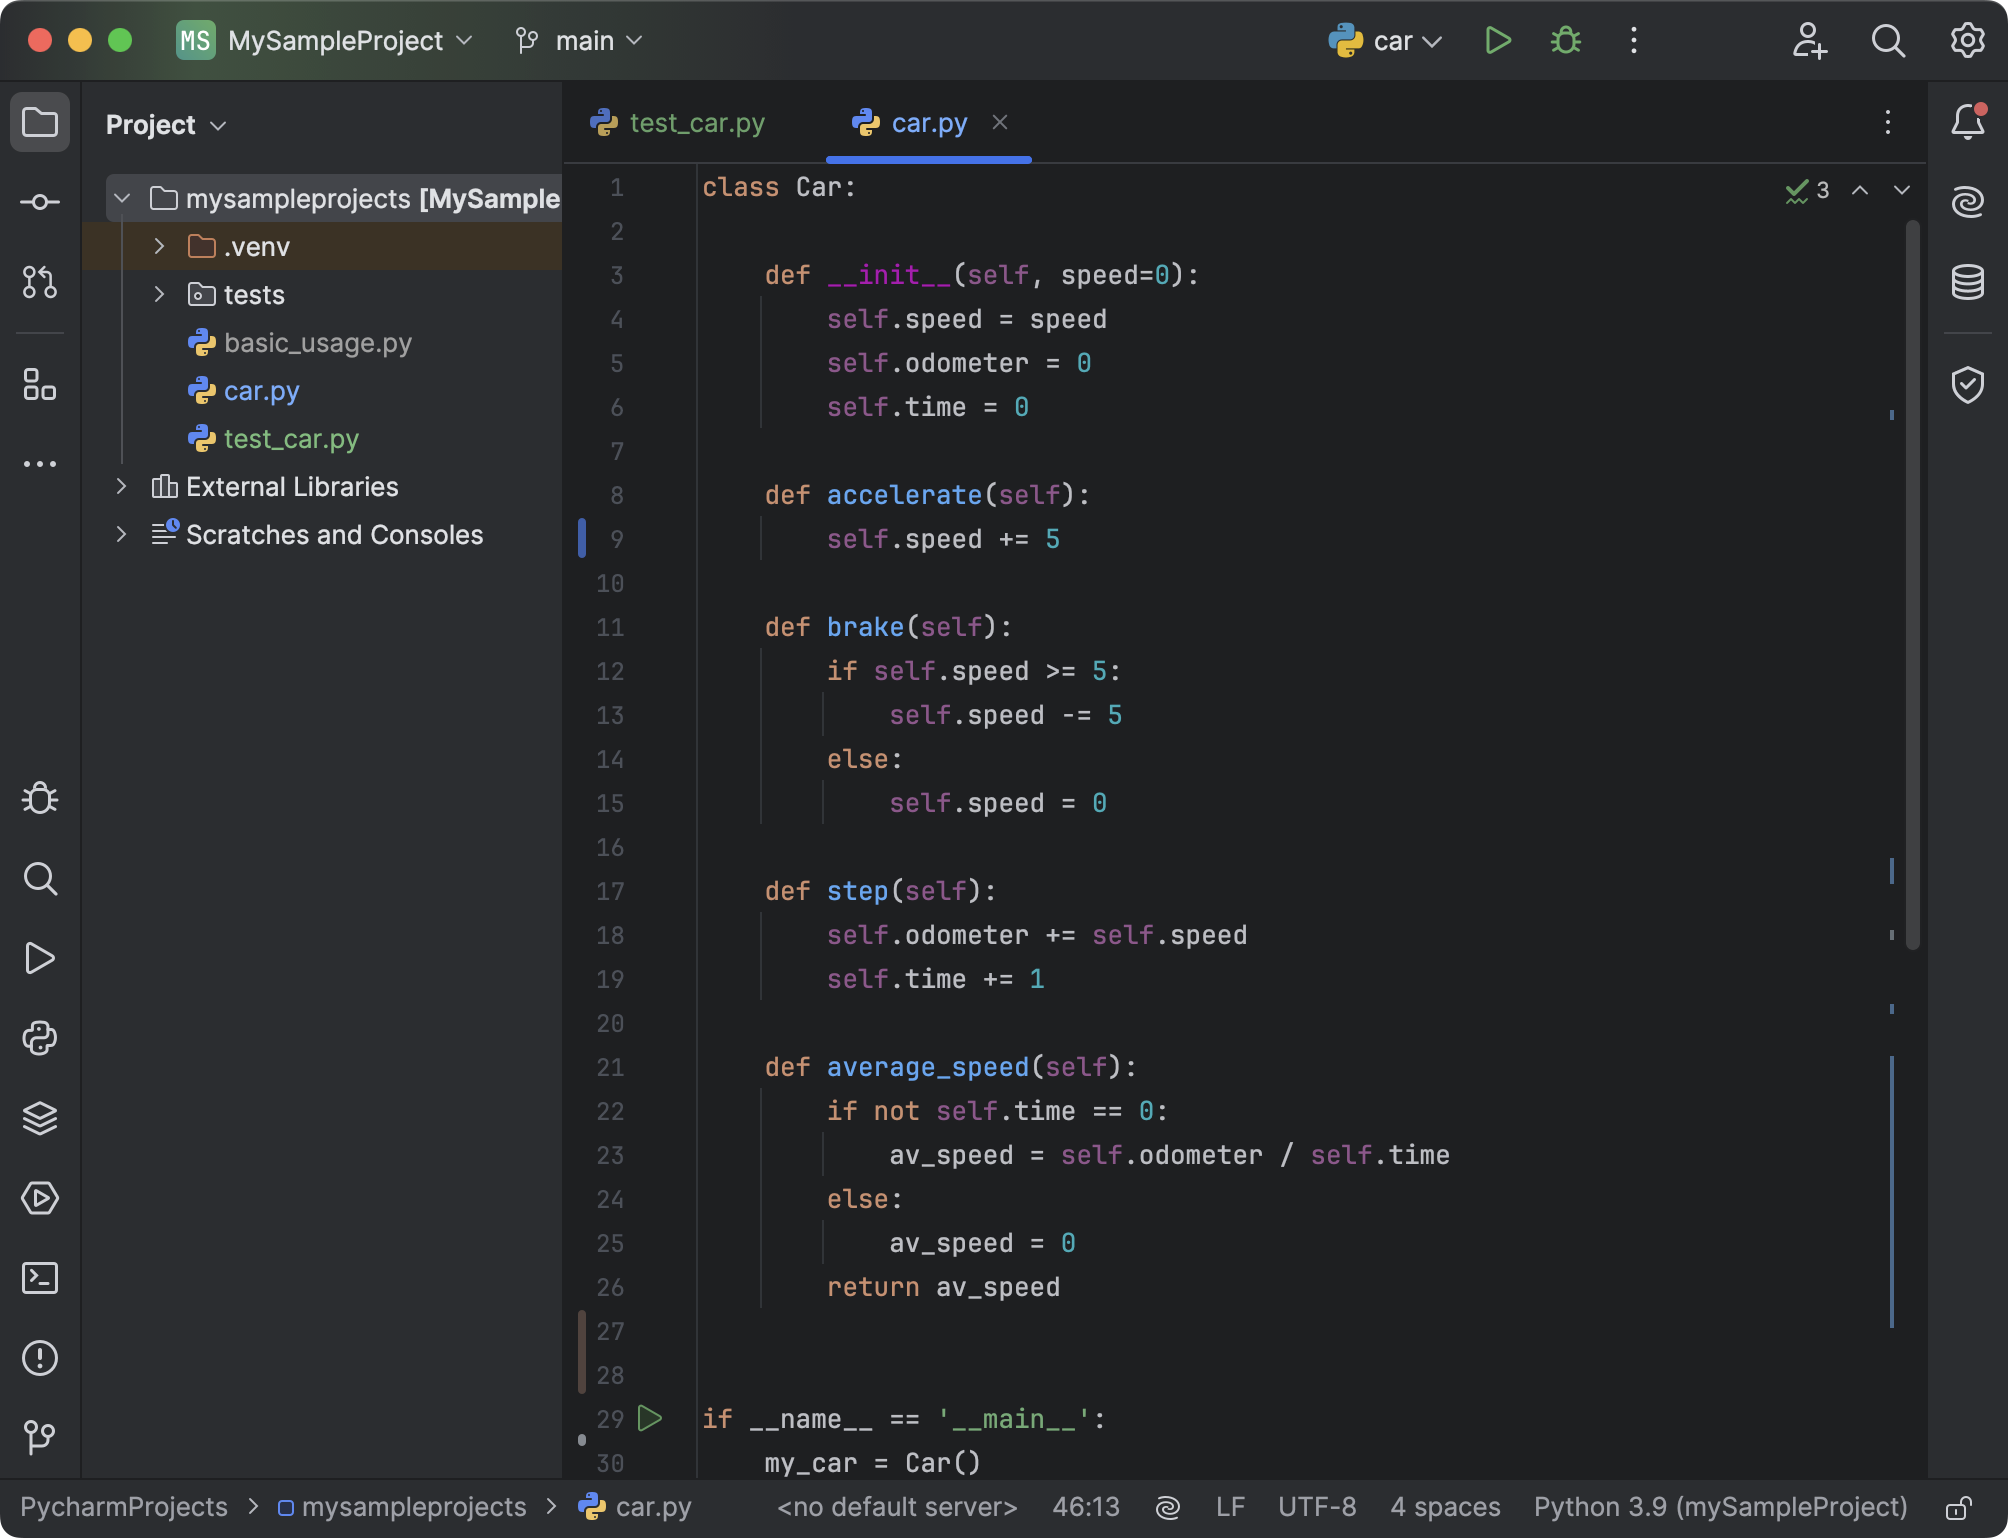
\includegraphics[width=0.8\textwidth]{figuras/pycharm.png} 
    \par 
    \small Fonte: (JETBRAINS, 2025)
\end{figure}


A seleção de um Ambiente de Desenvolvimento Integrado (IDE) é uma decisão fundamental que impacta a produtividade, a qualidade do código e a reprodutibilidade de um projeto de software. Para este trabalho, a escolha recaiu sobre o PyCharm, em detrimento de editores de código mais leves e genéricos, como o Visual Studio Code (VS Code). Essa decisão foi estratégica e baseada em uma análise das necessidades específicas de um projeto de machine learning de escopo acadêmico.

Enquanto o VS Code se destaca por sua leveza e versatilidade como um editor poliglota, sua funcionalidade para um ecossistema específico como o de Python depende da instalação e configuração manual de um conjunto de extensões para emular a experiência de um IDE.

O PyCharm, por outro lado, foi concebido especificamente para o desenvolvimento em Python, oferecendo uma experiência "out-of-the-box" coesa e otimizada, com todas as ferramentas essenciais pré-integradas e configuradas.

Em um projeto com prazo definido, como um Trabalho de Conclusão de Curso, o tempo economizado na configuração do ambiente de desenvolvimento pode ser reinvestido na lógica do problema, na experimentação e na análise de resultados.

\begin{figure}[H]
    \centering
    \caption{Exemplo da integração do PyCharm com Jupyter Notebooks.}
    \label{fig:jupyter}
    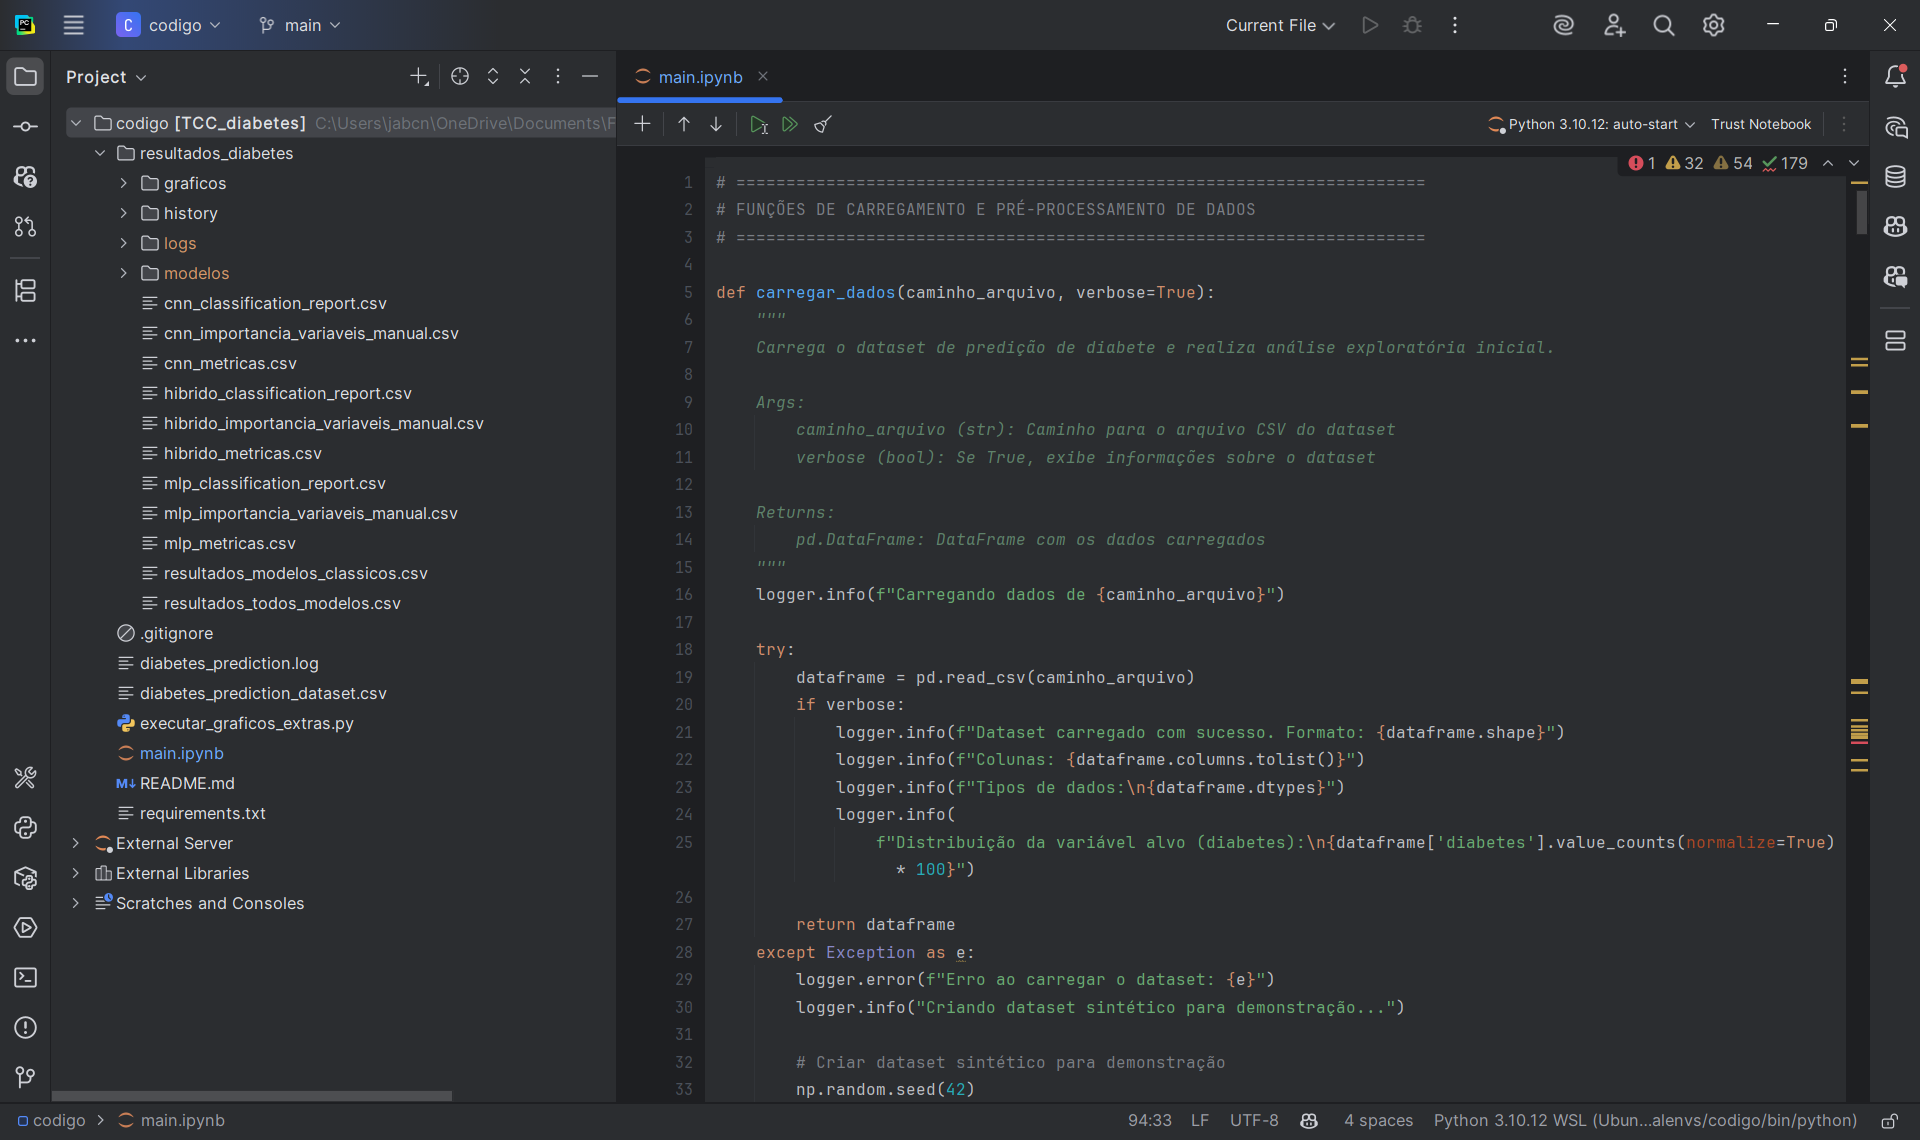
\includegraphics[width=0.8\textwidth]{figuras/jupyter.png} 
    \par 
    \small Fonte: Elaborado pelo autor.
\end{figure}

Três fatores foram preponderantes para esta escolha:

\textbf{Depuração e Introspecção de Código:} A complexidade de um pipeline de machine learning, que envolve múltiplas etapas de transformação de dados, treinamento de modelos e avaliação, torna a capacidade de depuração um requisito não-negociável. O depurador visual do PyCharm é nativamente superior para a ciência de dados. Ele permite a inspeção interativa de estruturas de dados complexas, como Data Frames do Pandas e arrays do NumPy, diretamente na interface gráfica durante a execução do código. A facilidade para definir breakpoints condicionais e executar o código passo a passo de forma intuitiva supera a experiência oferecida por configurações baseadas em extensões no VS Code, onde a depuração pode ser menos fluida.

\textbf{Gerenciamento de Ambiente e Reprodutibilidade:} A reprodutibilidade é um pilar da validade científica. O PyCharm oferece uma integração robusta para o gerenciamento de ambientes virtuais. A criação do ambiente, a ativação e a gestão de pacotes e suas versões são realizadas através de uma interface gráfica intuitiva, o que minimiza a probabilidade de erros de configuração. Esta abordagem garante que o ambiente de execução do projeto seja consistente, isolado e facilmente replicável por terceiros, um aspecto crucial para a validação dos resultados apresentados.

\textbf{Integração com Ferramentas Científicas:} A edição Profissional do PyCharm, utilizada neste projeto, oferece integração nativa com Jupyter Notebooks, conforme ilustrado na figura \ref{fig:jupyter}. Isso possibilita um fluxo de trabalho híbrido e eficiente: a fase de Análise Exploratória de Dados pode ser conduzida de forma interativa em um notebook para rápida visualização e experimentação, enquanto o código de produção do pipeline é desenvolvido e depurado nos módulos .py padrão. Manter essas duas atividades dentro de um único ambiente coeso elimina a fricção de alternar entre diferentes ferramentas.

Em suma, a escolha do PyCharm não foi uma questão de preferência pessoal, mas uma decisão de engenharia que visa mitigar riscos. Ao prover um ambiente coeso e pré-configurado, ele reduz a carga cognitiva do desenvolvedor, permitindo um foco maior na lógica do problema em vez de na configuração e manutenção das ferramentas de desenvolvimento. Esta abordagem eleva a qualidade e a robustez do trabalho, alinhando-o com boas práticas de engenharia de software.

\section{Python e Bibliotecas para Machine Learning}
Python é uma linguagem de programação de alto nível, de sintaxe simples e intuitiva, amplamente utilizada na ciência de dados e em projetos de inteligência artificial. Sua popularidade nessa área decorre, principalmente, do extenso ecossistema de bibliotecas especializadas, que simplificam as etapas do desenvolvimento de modelos de Machine Learning. A seguir, destacam-se algumas das principais tecnologias que compõem esse universo:

\subsection{Pandas}
Para a manipulação de dados estruturados, como o conjunto de dados de diabetes em formato CSV utilizado neste estudo, a biblioteca Pandas é o padrão da indústria e a escolha pragmática. Esta decisão foi tomada após a consideração de alternativas mais recentes e focadas em performance, como a biblioteca Polars.

O Pandas é uma biblioteca fundamental para manipulação e análise de dados. Ele fornece estruturas de dados eficientes, como Data Frames, que facilitam tarefas como limpeza, transformação, filtragem e agregação de dados, essenciais para o preparo das bases antes do treinamento dos modelos.\cite{McKinney2010} 

Ainda segundo McKinney\cite{McKinney2010} a biblioteca oferece uma interface flexível para lidar com conjuntos de dados variados, disponibilizando recursos como agregação e visualização de dados, de forma intuitiva e eficiente. 

A análise comparativa entre Pandas e Polars revela um clássico trade-off de engenharia de software. O Polars, implementado em Rust e projetado para paralelismo, oferece uma performance de execução significativamente superior, especialmente em operações de leitura/escrita e em datasets de grande volume. No entanto, o conjunto de dados deste projeto, com 100.000 instâncias, não é grande o suficiente para que a performance do Pandas se torne um gargalo crítico. O tempo de execução do pipeline de pré-processamento com Pandas permanece na ordem de segundos ou poucos minutos, o que é perfeitamente aceitável para o projeto.

Neste contexto, a decisão de utilizar Pandas foi motivada pela otimização de um recurso mais escasso e valioso: o tempo de desenvolvimento. As vantagens do Pandas que justificaram sua escolha foram:

\textbf{Maturidade e Integração do Ecossistema:} A principal fortaleza do Pandas é sua integração nativa e transparente com as demais bibliotecas do projeto. Scikit-learn, Matplotlib e Seaborn foram desenvolvidos para interagir diretamente com as estruturas de dados do Pandas. Utilizar Polars exigiria conversões explícitas para o formato Pandas antes de passar os dados para essas bibliotecas, adicionando complexidade desnecessária, verbosidade ao código e um potencial ponto de falha no pipeline.

\textbf{Produtividade e Suporte Comunitário:} Sendo a ferramenta mais estabelecida, o Pandas possui uma vasta base de conhecimento, incluindo documentação oficial detalhada, inúmeros tutoriais e uma comunidade massiva que fornece soluções para praticamente qualquer problema de manipulação de dados. Essa riqueza de recursos acelera significativamente o desenvolvimento e a depuração, um fator crucial em projetos com cronogramas definidos.

O Pandas foi a espinha dorsal de toda a fase de exploração e pré-processamento de dados, com sua lógica centralizada no módulo de processamento de dados do projeto. Suas funcionalidades foram essenciais para:

\begin{itemize}
    \item \textbf{Carregamento de Dados:} Ler o conjunto de dados original do arquivo CSV para um Data Frame.
    \item \textbf{Análise Exploratória de Dados (EDA):} Utilizar métodos nativos da biblioteca para obter uma compreensão inicial da estrutura, qualidade e distribuição dos dados.
    \item \textbf{Limpeza e Transformação:} Executar operações de limpeza, como a renomeação de colunas para o português e o tratamento de variáveis categóricas através de técnicas como
    \item \textbf{Engenharia de Features:} Criar, modificar ou remover colunas para preparar o conjunto de dados para os modelos de machine learning.
    \item \textbf{Segmentação dos Dados:} Separar o Data Frame principal em um conjunto de variáveis preditoras (X) e a variável alvo (y), que é o formato padrão para a maioria das APIs de machine learning.
\end{itemize}

Portanto, a escolha do Pandas reflete uma decisão que priorizou a velocidade de desenvolvimento, a robustez da integração e a minimização do atrito entre as ferramentas em detrimento de uma otimização de performance de execução que traria benefícios marginais para a escala do problema em questão.

\subsection{NumPy}
A inclusão da biblioteca NumPy no projeto não representa uma escolha entre alternativas, mas sim a adoção de um pilar fundamental e indispensável. O NumPy é o alicerce sobre o qual todo o ecossistema de ciência de dados em Python é construído. Bibliotecas cruciais utilizadas neste trabalho, como Pandas, Scikit-learn e Tensor Flow, dependem intrinsecamente da estrutura de dados central do NumPy, o ndarray, para realizar operações numéricas de alta performance.

A eficiência do NumPy deriva de sua implementação em linguagens de baixo nível, que permite a execução de operações matemáticas em vetores e matrizes de forma muito mais rápida do que seria possível com laços em Python puro. Tentar substituir o NumPy significaria abandonar o vasto e maduro ecossistema de ferramentas científicas de Python ou reconstruir funcionalidades básicas de computação numérica, ambas opções inviáveis para o escopo deste trabalho.

Ao longo do projeto a biblioteca operou de forma transparente nos bastidores em quase todas as etapas. Quando um DataFrame do Pandas era criado, suas colunas numéricas eram armazenadas internamente como arrays NumPy. Da mesma forma, quando os dados eram passados para os modelos do Scikit-learn ou Keras para treinamento e predição, a estrutura de dados subjacente manipulada por esses frameworks era o ndarray do NumPy.

Em momentos específicos, a biblioteca foi invocada diretamente. No módulo de processamento de dados onde funções do NumPy foram utilizadas para realizar transformações matemáticas eficientes em colunas de dados. Além disso, na etapa final do pré-processamento, os dados preparados foram explicitamente convertidos para o formato de array NumPy, que é o formato de entrada padrão e otimizado exigido pela maioria dos algoritmos de machine learning, incluindo os implementados pelo Keras e Scikit-learn.

\subsection{Matplotlib e Seaborn}
A estratégia de visualização de dados para este trabalho foi deliberadamente focada na geração de gráficos estáticos de alta qualidade, utilizando a combinação sinérgica das bibliotecas Matplotlib e Seaborn. A escolha desta abordagem foi diretamente influenciada pelo meio de comunicação primário dos resultados do projeto: um documento de tese estático.

Foram consideradas alternativas como Plotly e Bokeh, bibliotecas que se destacam pela capacidade de criar visualizações interativas, ideais para dashboards e aplicações web. No entanto, a principal vantagem dessas ferramentas é a interatividade que é completamente perdida quando um gráfico é incorporado em um documento de texto ou PDF. A exportação de um gráfico interativo como uma imagem estática frequentemente resulta em uma qualidade visual inferior e menor controle sobre a formatação final em comparação com um gráfico gerado nativamente para esse propósito, temos um exemplo na figura \ref{fig:matplotlib}.

\begin{figure}[H]
    \centering
    \caption{Exemplo de gráfico gerado com Matplotlib.}
    \label{fig:matplotlib}
    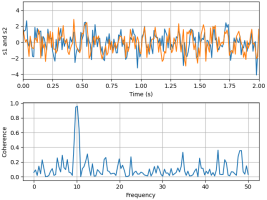
\includegraphics[width=0.8\textwidth]{figuras/matplotlib_example.png} 
    \par 
    \small Fonte: matplotlib(2025))
\end{figure}

O que justifica a escolha do Matplotlib e Seaborn pela complementaridade de suas funções:

\textbf{Matplotlib como a Fundação Flexível:} Matplotlib é a biblioteca de visualização mais fundamental e poderosa do ecossistema Python. Ela oferece um controle granular e de baixo nível sobre todos os elementos de uma figura como eixos, títulos, legendas, cores, fontes e anotações.

\textbf{Seaborn para Produtividade e Estética Estatística:} Seaborn funciona como uma API de alto nível construída sobre o Matplotlib. Sua principal função é simplificar a criação de gráficos estatísticos complexos e estéticamente agradáveis. Para a fase de Análise Exploratória de Dados, o Seaborn acelera drasticamente a obtenção de insights ao permitir a geração de visualizações ricas, como mapas de calor de correlação, gráficos de distribuição e diagramas de dispersão, frequentemente com uma única linha de código.

A combinação das duas ferramentas oferece uma solução ótima juntando a velocidade e a simplicidade do Seaborn para a exploração inicial e a criação de gráficos padrão, e o poder de personalização do Matplotlib para os ajustes finos necessários para garantir que as figuras finais sejam informativas, precisas e visualmente claras. Essa abordagem demonstra um entendimento de que a visualização de dados não é apenas uma ferramenta de análise para o pesquisador, mas também um instrumento de comunicação para a audiência, onde a clareza e a adequação ao meio são primordiais.

\subsection{Scikit Learn}
A biblioteca Scikit learn é um dos principais frameworks para o desenvolvimento e a avaliação de modelos de Machine Learning tradicionais. Ela fornece algoritmos para classificação, regressão, clustering e redução de dimensionalidade, além de ferramentas para validação cruzada, seleção de atributos e ajuste de hiperparâmetros\cite{Pedregosa2011}. 

A utilização da biblioteca Scikit-learn foi uma decisão metodológica fundamental para atender a um dos objetivos específicos do projeto: "Comparar a precisão do modelo proposto com métodos alternativos". A sua inclusão não foi opcional, mas sim um requisito para garantir o rigor científico da análise comparativa.

Scikit-learn é o framework padrão de fato para algoritmos de machine learning clássicos em Python. Sua escolha se baseia em três pilares:

\textbf{Padrão da Indústria e API Consistente:} A biblioteca oferece uma implementação robusta e otimizada de uma vasta gama de algoritmos de classificação, regressão e clusterização. Mais importante, ela o faz através de uma API consistente e unificada, que simplifica enormemente o processo de treinar e avaliar múltiplos modelos de forma comparável.

\textbf{Estabelecimento de um Baseline Científico:} Antes de justificar o uso de um modelo mais complexo e computacionalmente mais caro, como uma rede neural artificial, é uma prática essencial na pesquisa estabelecer um baseline de performance. Modelos mais simples e interpretáveis, como Regressão Logística ou Random Forest, fornecidos pelo Scikit-learn, servem como um ponto de referência crucial. Eles ajudam a quantificar a dificuldade intrínseca do problema e a determinar se a complexidade adicional de uma rede neural se traduz em um ganho de desempenho significativo.

\textbf{Ferramentas de Avaliação Padronizadas:} O módulo sklearn.metrics é considerado o padrão-ouro para a avaliação de modelos de machine learning. Ele fornece implementações eficientes e amplamente validadas de todas as métricas de desempenho críticas mencionadas no trabalho, como Acurácia, Precisão, Recall, F1-Score e a Matriz de Confusão. Utilizar este módulo para avaliar todos os modelos, incluindo a rede neural implementada com Keras, garante que a comparação seja justa, consistente e baseada em métricas calculadas de forma idêntica, eliminando vieses de implementação.

\section{Tensor Flow e Keras}
Para projetos que demandam aprendizado profundo, as bibliotecas Tensor Flow e Keras são amplamente utilizadas. O Tensor Flow, desenvolvido pela Google, oferece uma infraestrutura robusta para o treinamento de modelos complexos de redes neurais, enquanto o Keras, integrável ao Tensor Flow, fornece uma interface mais amigável, facilitando a definição e o treinamento de modelos de Deep Learning.

A decisão da escolha pela a API de alto nível Keras, utilizando o Tensor Flow como seu backend de computação foi tomada após uma análise comparativa com a principal alternativa no campo de deep learning, o PyTorch.

PyTorch é amplamente reconhecido por sua flexibilidade, sua API e seu grafo computacional dinâmico, características que o tornam a ferramenta preferida em ambientes de pesquisa acadêmica, onde a experimentação com novas e complexas arquiteturas de rede é comum. Keras, em contraste, foi desenvolvido com uma filosofia de simplicidade, modularidade e facilidade de uso, abstraindo grande parte da complexidade de baixo nível associada ao treinamento de redes neurais.

A escolha de Keras e Tensor Flow foi estratégica e alinhada ao escopo do projeto:

\textbf{Foco na Aplicação, Não na Pesquisa de Arquiteturas:} O objetivo deste TCC é a aplicação de uma arquitetura de rede neural conhecida como Perceptron de Múltiplas Camadas - MLP para resolver um problema prático, e não a pesquisa e o desenvolvimento de uma nova topologia de rede. Neste contexto, a abstração e a simplicidade do Keras são uma vantagem competitiva. Elas permitem que o desenvolvedor se concentre naquilo que é mais importante para o problema: a definição da arquitetura número de camadas, neurônios, funções de ativação e o ajuste de hiperparâmetros, em vez de se preocupar com a implementação manual de laços de treinamento, cálculo de gradientes e atualização de pesos, tarefas que são mais explícitas em PyTorch.

\textbf{Produtividade e Curva de Aprendizagem:} Em um projeto de graduação com um cronograma definido, a produtividade é um fator crítico. A curva de aprendizagem mais suave do Keras permite que um desenvolvedor se torne produtivo muito mais rapidamente. A capacidade de construir, compilar e treinar um modelo com poucas linhas de código declarativo acelera o ciclo de experimentação, permitindo que mais tempo seja dedicado à análise dos resultados e ao refinamento do modelo.

A utilização conjunta de Scikit-learn e Keras constitui uma estratégia metodológica complementar e robusta. O Scikit-learn foi usado para estabelecer o piso de performance com modelos clássicos, definindo o baseline a ser superado. O Keras, por sua vez, foi empregado para testar a hipótese central do trabalho: que uma abordagem de deep learning, apesar de sua maior complexidade, poderia oferecer um desempenho preditivo superior para este problema específico. Essa dualidade de ferramentas transforma a seleção tecnológica em um desenho experimental estruturado, com um grupo de controle e um grupo de teste.

\section{Limitações e Ética}
A adoção de sistemas baseados em inteligência artificial na saúde exige atenção a diversas limitações e questões éticas. Devem ser considerados o respeito à privacidade e à confidencialidade dos dados dos pacientes, além das possíveis vieses presentes nos dados utilizados para o treinamento, que podem resultar em discriminações ou erros sistemáticos. Outro ponto relevante é a necessidade de transparência na interpretação dos resultados produzidos pelo modelo. A conformidade com normas éticas e regulatórias, bem como a análise criteriosa dos resultados preditivos por profissionais de saúde, são fundamentais para o uso responsável dessas tecnologias \cite{BRASIL2022}.

O trabalho desenvolvido tem como objetivo principal criar uma ferramenta de apoio ao profissional de saúde. Ressalta-se que essa ferramenta não substitui o profissional nem deve ser utilizada como diagnóstico final, mas sim como um auxílio adicional no processo de tomada de decisão clínica.
